\section{Charged Kaon Decays at the Super Proton Synchrotron}
\label{sec:na48_na62_experiment}
NA48/2~\cite{Batley:1999fv} and NA62~\cite{Martellotti:2015kna} (also known as NA48/3) are two experiments studying rare kaon decays at the CERN Super Proton Synchrotron (SPS).
Each has own objective, but both study kaon decays and have a dedicated $K^+$ beam which we can take advantage of for the purpose of setting limits.
Note that the beam is actually a simultaenous $K^+$ and $K^-$ beam, but there are some advantages that we will make use of that make the $K^+$ beam more desirable.
The charged kaon beam is produced similarly as the muon beam was describe in the previous section.
Protons are collided with targets which produce a secondary beam, which are steered towards a target after being selected to ensure that the beam content is pure kaon.
For a target, beryllium is used.
The proton beam used is a $400\textrm{GeV}$ beam.

\subsection{NA48/2}
The first experiment of the two finished taking data in 2004, yet limits on new physics can still be done using the data collected on tape.
NA48/2 is based on the upgraded NA48 experiment, and was primarily designed to look for charge-parity (CP) violation in the decays of the charged kaons:

\begin{align}
K^\pm & \rightarrow \pi^+ + \pi^- + \pi^\pm \\
K^\pm & \rightarrow \pi^0 + \pi^0 + \pi^\pm
\end{align}

The experiment collected $1.0 \times 10^{11}$ $K^+$ decays inside its fiducial volume during its running time from $2003-2004$.
All the data stored on tape is still being used to put some of the most competitive limits on the dark photon parameter space, and has recently ruled it out as a candidate for the $(g-2)_\mu$ discrepancy~\cite{Goudzovski:2014rwa}.
For the most part of this analysis, we will be treating NA48/2 as the NA62 experiment with a scaled down number of kaons decaying in the fiducial volume, as we are most interested in setting limits for the upcoming experiment.

\subsection{NA62}
On the other hand, NA62 is looking to measure the Cabbibo-Kobayashi-Maskawa (CKM) matrix element $|V_{td}|$ at the level of $10\%$ by measuring the very rare charged kaon decay:
\begin{equation}
K^+ \rightarrow \pi^+ + \nu + \bar{\nu}
\end{equation}
This branching ratio in the SM comes at $\textrm{BR}(K^+ \rightarrow \pi^+ + \nu + \bar{\nu}) = (7.81 \pm 0.75 \pm 0.29) \times 10^{-11}$, with the first uncertainty being due to the uncertain input parameters, and the second uncertainty being due to theoretical uncertainty~\cite{Straub:2010ih}.
The relative size of this branching ratio should allow one to put strong limits on any new physics involving the charged kaons.
In October 2014, NA62 successfully launched and began taking data.

Different than the previous experiments, NA62 is analyzing kaon decays while they are in flight with momentum of the $K^+$ beam at $75\textrm{GeV}$.
This beam momentum is well defined, having an error of $1\%$.
The liquid krypton electro-magnetic calorimeter (LKr) is reused from the NA48 experiments and sits past the fiducial volume, and has a coverage from the beam of $8.5\textrm{mrad}$.
New to this experiment is the Muon Veto (MUV) and the Large-Angle Photon Vetoes (LAV).
The LAV provides coverage from the LKr limit of $8.5\textrm{mrad}$ up to $50\textrm{mrad}$, and has an inefficiency of $10^{-3} - 10^{-4}$ on detecting photons with energies down to $150\textrm{MeV}$.
The MUV is used to reject muons, which is also handled by the Ring Imaging CHerenkov detector (RICH).
There are many other important components to the experiment, but the most important things we must consider are the beam momentum, the LKr, and the photon veto efficiency.

A schematic view of the experiment is laid out in Fig.~\ref{fig:na62_experiment}.

\begin{figure}[h]
    \centering
    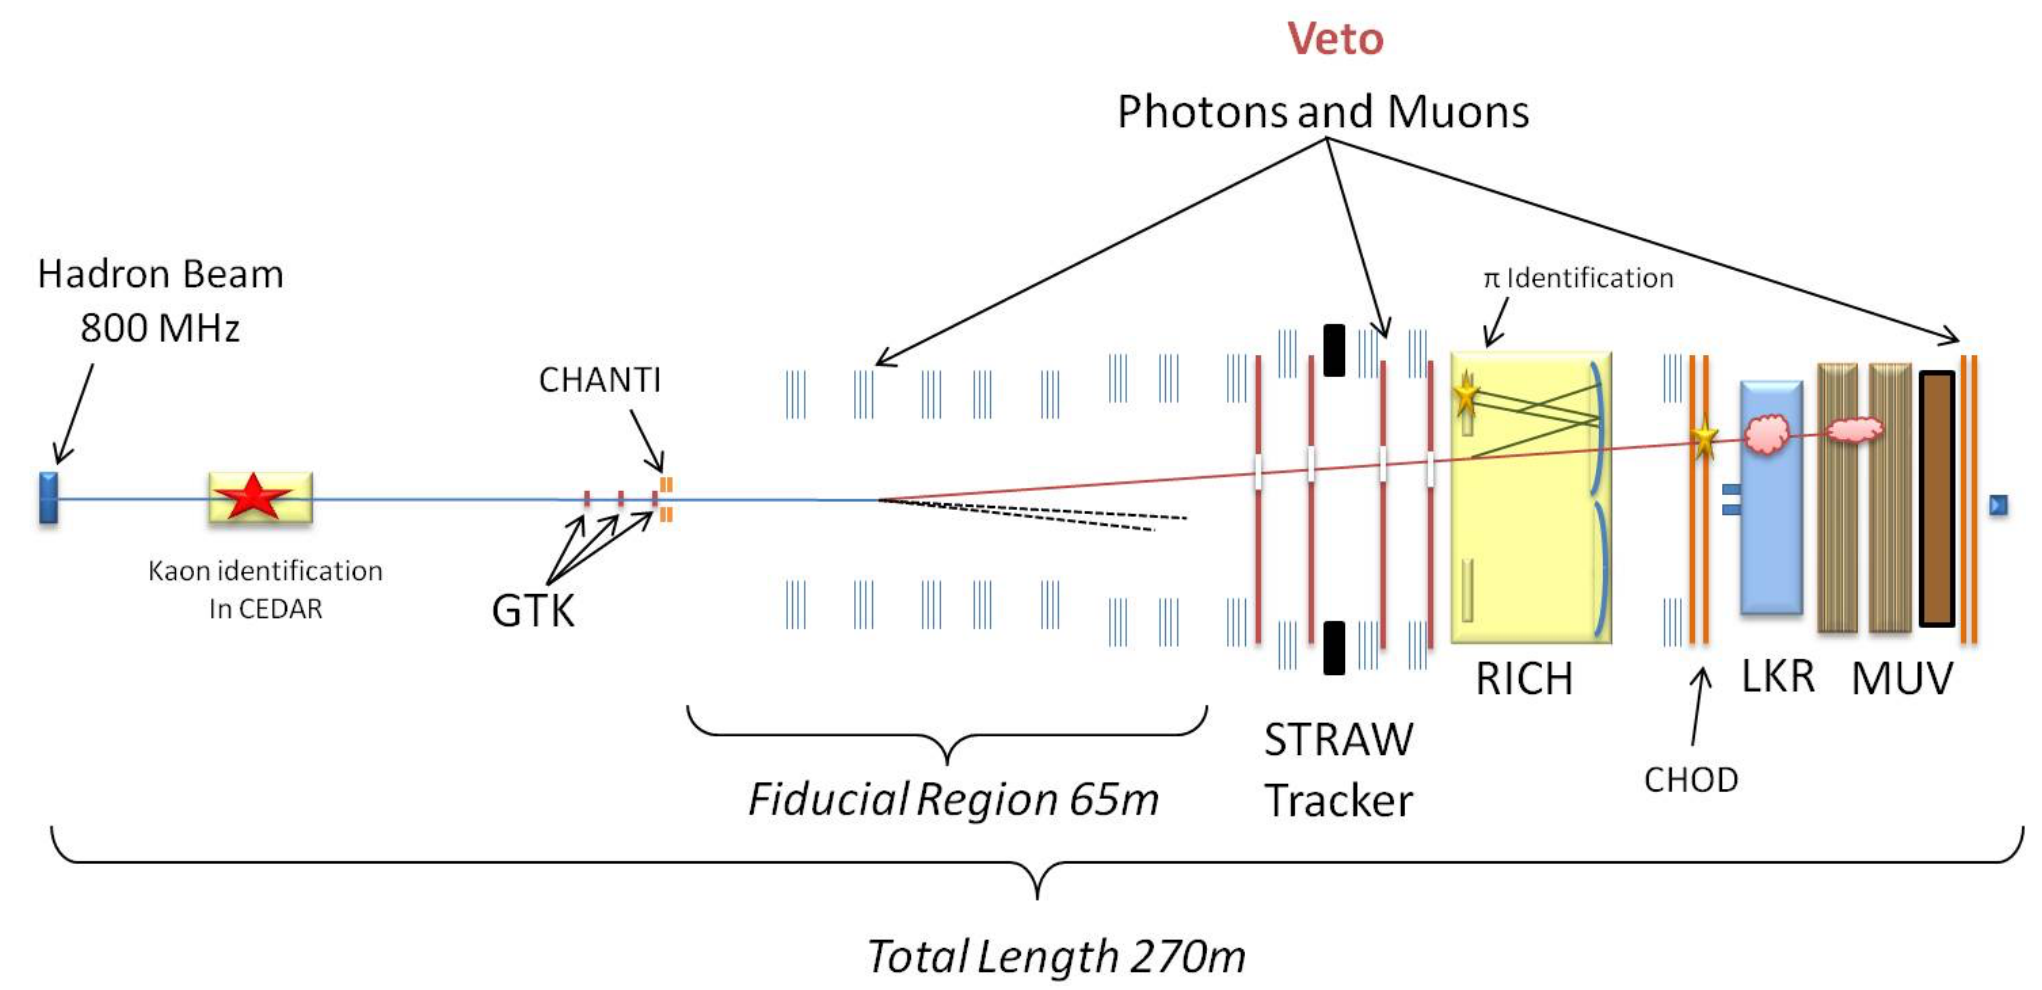
\includegraphics[width=\textwidth]{Figures/experiments/na62_schematic}
    \caption{Schematic of the NA62 experiment from~\cite{Martellotti:2015kna}. The beam collides with a beryllium target and is then identified for kaons. $K^+$ decays that are visible will decay within the fiducial volume and be captured by the LKr.}
    \label{fig:na62_experiment}
\end{figure}
